\documentclass[11pt]{article}
\usepackage{hyperref}
\usepackage{subfigure}


\usepackage{hyperref}
\hypersetup{unicode=true, colorlinks, breaklinks, citecolor=blue, linkcolor=black}

\usepackage{xltxtra}
\usepackage{booktabs} 
\usepackage{subfigure}
\usepackage{graphicx}


\title{Data Mining Capstone Task 1}
%\author{Jiacheng Pan}

\begin{document}
\maketitle

\section{Abstract}
In this task, I used \emph{python} toolkits to perform the analysis, to get an overview of the topics of the reviews and the review star distribution.
In particular, I used packages such as \emph{gensim}, \emph{sklearn} for the topic extraction.

For data visualisation, I used \emph{D3} to do all the drawings.

\section{Implementations}
\subsection{Topic mining of all restaurant reviews (Task 1.1)}
To understand what people are talking about among the review data, I used topic model LDA to extract 10 topics from all the reviews that are for \emph{restaurants}.

I applied \emph{TfidfVectorizer} to vectorize the raw review data, after filtering all reviews and only collect those for restaurants.
The TF transformation was made to be linear, and I enabled IDF reweighting.
I specified the n-gram range to be 1 to 2, i.e. terms with 1 or two words were collected.

By using \emph{D3}, I applied \emph{word cloud} to visualise the data.
Essentially, each cloud represents a topic. The font size shows the significance of the corresponding term in this topic.
Ten colours are used to distinguish the topics.

Figure \ref{fig:all_topics} shows the result.

The result is also shown in \href{http://jiacheng-pan.me/standalone/datamining_capstone/task1/all_reviews_topics.html}{this link}.

\begin{figure}[htp!]
  \centering
  \subfigure[Topic 0] { 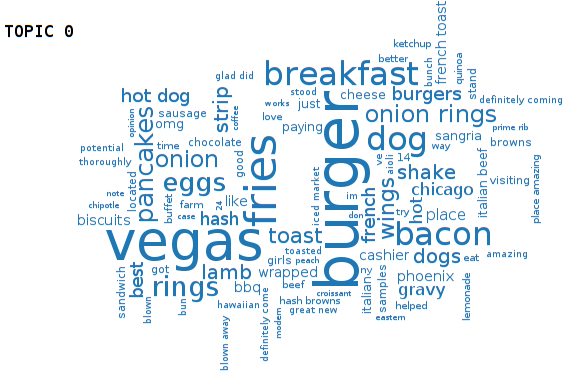
\includegraphics[width=0.35\textwidth]{./img/all_reviews/topic0.png} }
  \subfigure[Topic 1] { 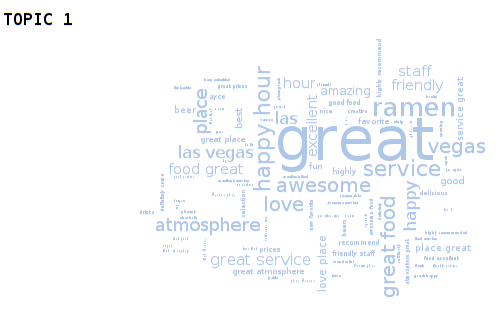
\includegraphics[width=0.35\textwidth]{./img/all_reviews/topic1.png} }
  \subfigure[Topic 2] { 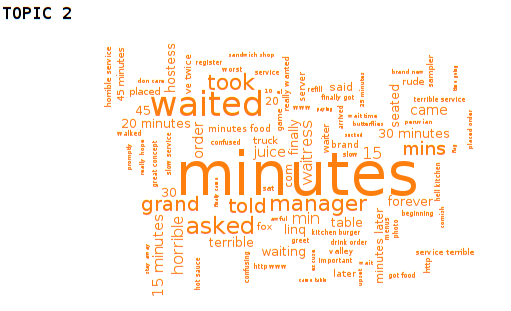
\includegraphics[width=0.35\textwidth]{./img/all_reviews/topic2.png} }
  \subfigure[Topic 3] { 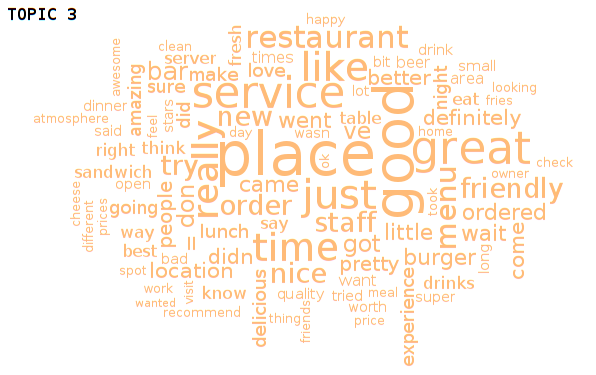
\includegraphics[width=0.35\textwidth]{./img/all_reviews/topic3.png} }
  \subfigure[Topic 4] { 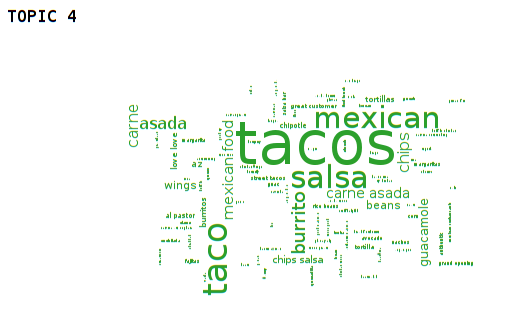
\includegraphics[width=0.35\textwidth]{./img/all_reviews/topic4.png} }
  \subfigure[Topic 5] { 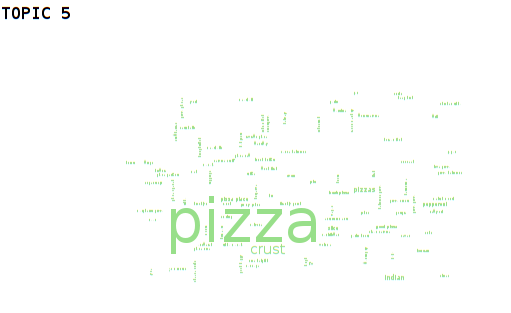
\includegraphics[width=0.35\textwidth]{./img/all_reviews/topic5.png} }
  \subfigure[Topic 6] { 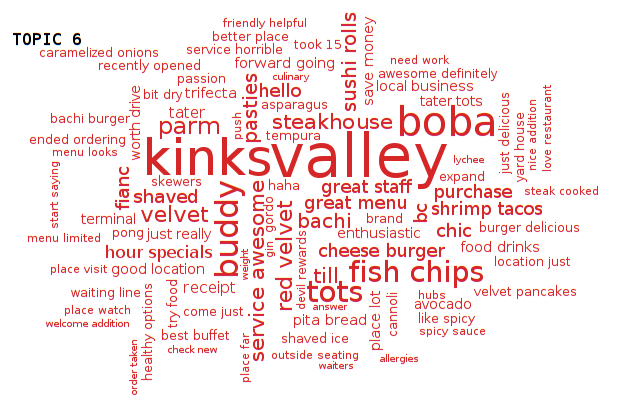
\includegraphics[width=0.35\textwidth]{./img/all_reviews/topic6.png} }
  \subfigure[Topic 7] { 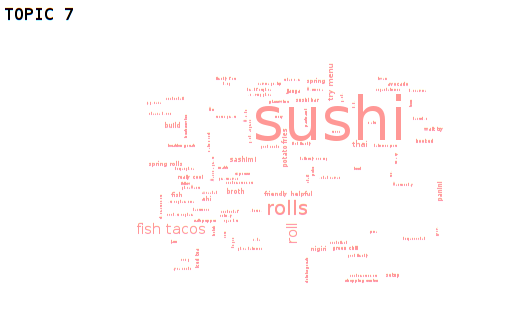
\includegraphics[width=0.35\textwidth]{./img/all_reviews/topic7.png} }
  \subfigure[Topic 8] { 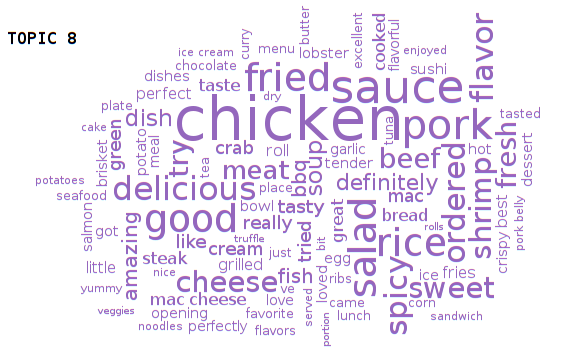
\includegraphics[width=0.35\textwidth]{./img/all_reviews/topic8.png} }
  \subfigure[Topic 9] { 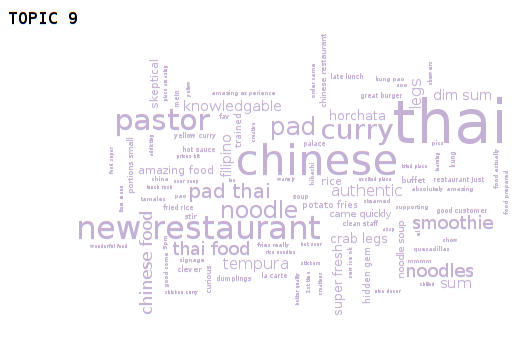
\includegraphics[width=0.35\textwidth]{./img/all_reviews/topic9.png} }
  \caption{Ten topics mined from all restaurant reviews}
  \label{fig:all_topics}
\end{figure}


Here are several observations:
\begin{enumerate}
  \item Cuisines / foods are very popular topics -- topics 4, 5, 7, 9 more or less emphesize a particular cuisine, e.g. Mexican tacos, pizza, Japanese sushi, and Thai / Chinese food, while topics 0, 6, 8 emphesize certain foods or drinkings.
  \item General comments (usually good) to the restaurants -- topics 1 and 3 clearly show a good impression, while topic 2 possibly suggests an inferior impression in terms of waiting (and then asking for managers). In particular, topic 2 also suggests that \emph{time} is a very important topic, or factor, when customers are reviewing a restaurant.
  \item Locations are also mentioned, especially "Las Vagas Valley", spreaded amongst topics 0, 1, 6.
\end{enumerate}


\subsection{Topic mining of positive and negative reviews (Task 1.2)}
In this task, I managed to explore the topic distribution for subsets of all the reviews.
In particular, this section introduces the observations made upon subsets of negative reviews (reviews with star number <= 2) and positive reviews (reviews with star number >= 4).

The topic model used is still LDA, with identical configurations as in task 1.1.

Figures \ref{fig:neg_topics} and \ref{fig:pos_topics} show the result.

The result is also shown in
\href{http://jiacheng-pan.me/standalone/datamining_capstone/task1/pos_reviews_topics.html}{this link (positive views)}
and 
\href{http://jiacheng-pan.me/standalone/datamining_capstone/task1/neg_reviews_topics.html}{this link (negative views)}.

\begin{figure}[htp!]
  \centering
  \subfigure[Topic 0] { 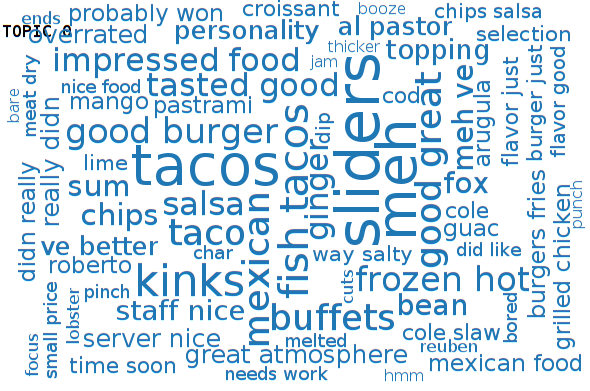
\includegraphics[width=0.35\textwidth]{./img/neg_reviews/neg_topic0.png} }
  \subfigure[Topic 1] { 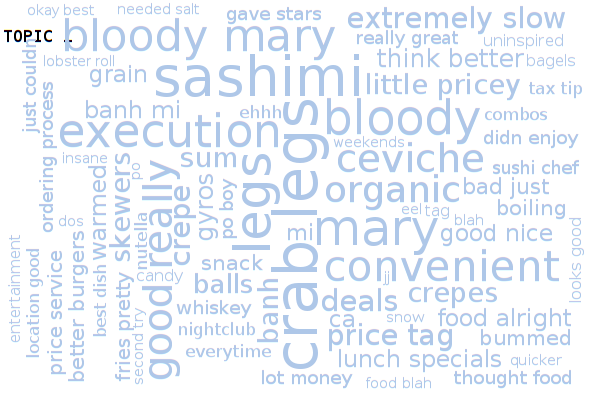
\includegraphics[width=0.35\textwidth]{./img/neg_reviews/neg_topic1.png} }
  \subfigure[Topic 2] { 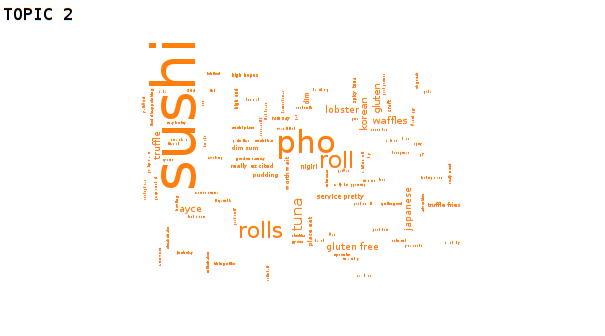
\includegraphics[width=0.35\textwidth]{./img/neg_reviews/neg_topic2.png} }
  \subfigure[Topic 3] { 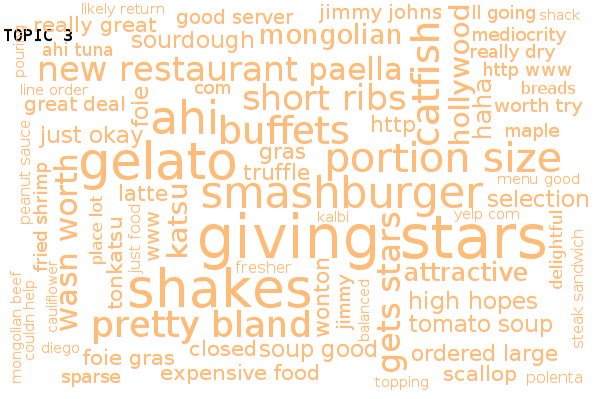
\includegraphics[width=0.35\textwidth]{./img/neg_reviews/neg_topic3.png} }
  \subfigure[Topic 4] { 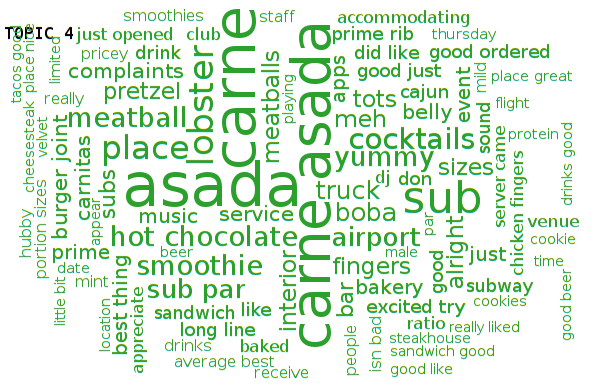
\includegraphics[width=0.35\textwidth]{./img/neg_reviews/neg_topic4.png} }
  \subfigure[Topic 5] { 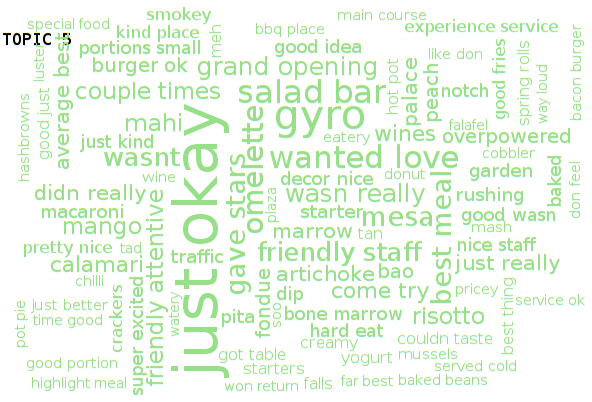
\includegraphics[width=0.35\textwidth]{./img/neg_reviews/neg_topic5.png} }
  \subfigure[Topic 6] { 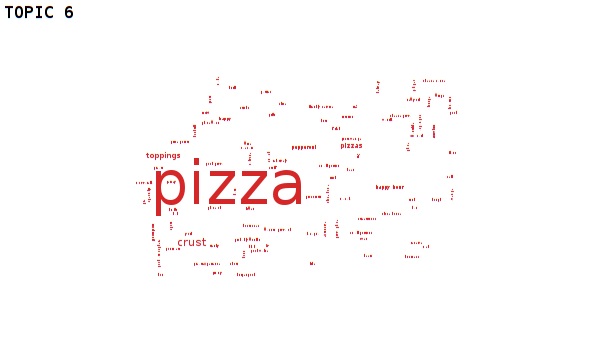
\includegraphics[width=0.35\textwidth]{./img/neg_reviews/neg_topic6.png} }
  \subfigure[Topic 7] { 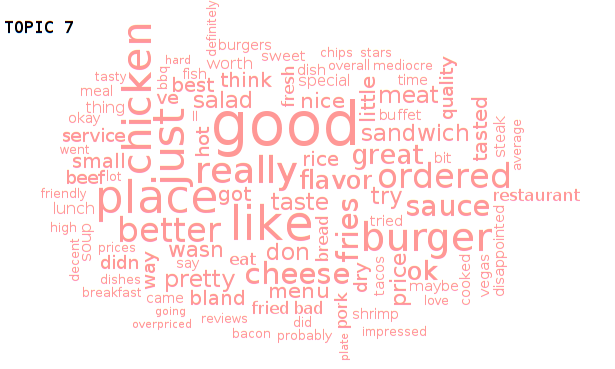
\includegraphics[width=0.35\textwidth]{./img/neg_reviews/neg_topic7.png} }
  \subfigure[Topic 8] { 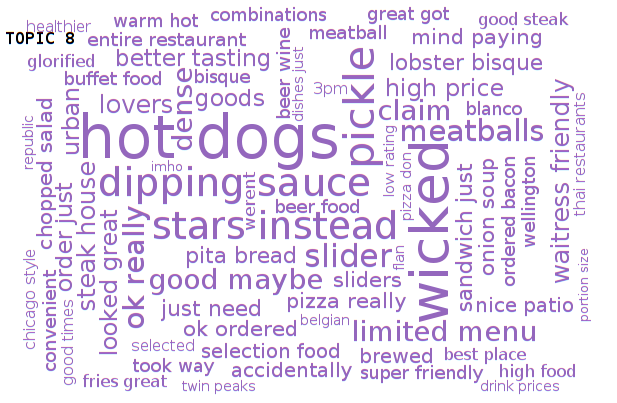
\includegraphics[width=0.35\textwidth]{./img/neg_reviews/neg_topic8.png} }
  \subfigure[Topic 9] { 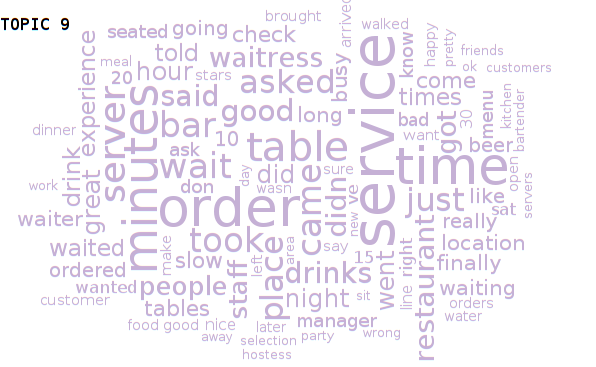
\includegraphics[width=0.35\textwidth]{./img/neg_reviews/neg_topic9.png} }
  \caption{Ten topics mined from negative restaurant reviews}
  \label{fig:neg_topics}
\end{figure}

\begin{figure}[htp!]
  \centering
  \subfigure[Topic 0] { 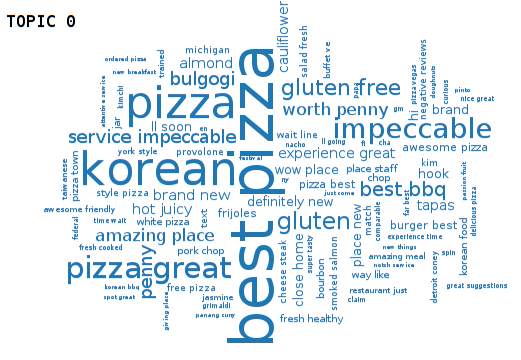
\includegraphics[width=0.35\textwidth]{./img/pos_reviews/pos_topic0.png} }
  \subfigure[Topic 1] { 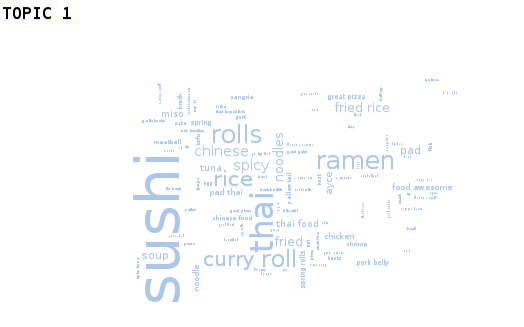
\includegraphics[width=0.35\textwidth]{./img/pos_reviews/pos_topic1.png} }
  \subfigure[Topic 2] { 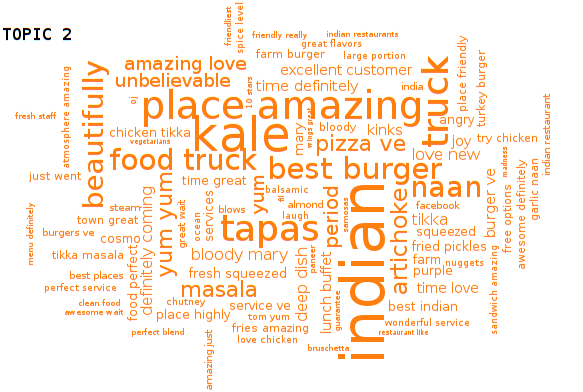
\includegraphics[width=0.35\textwidth]{./img/pos_reviews/pos_topic2.png} }
  \subfigure[Topic 3] { 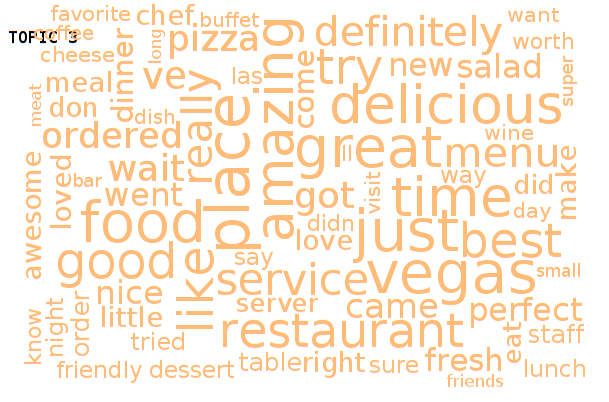
\includegraphics[width=0.35\textwidth]{./img/pos_reviews/pos_topic3.png} }
  \subfigure[Topic 4] { 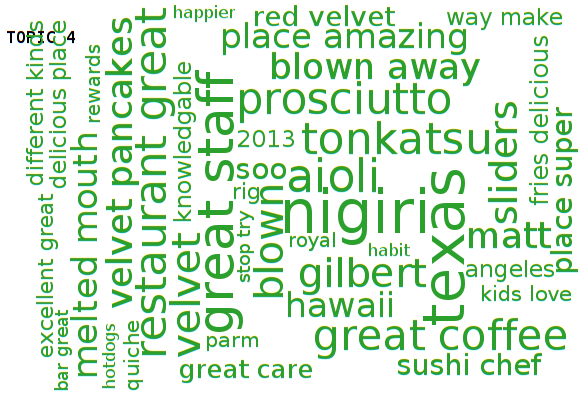
\includegraphics[width=0.35\textwidth]{./img/pos_reviews/pos_topic4.png} }
  \subfigure[Topic 5] { 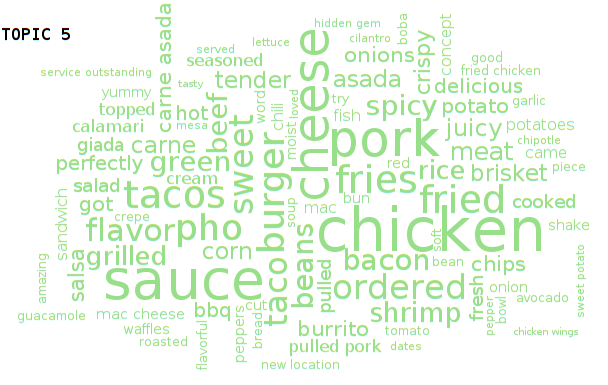
\includegraphics[width=0.35\textwidth]{./img/pos_reviews/pos_topic5.png} }
  \subfigure[Topic 6] { 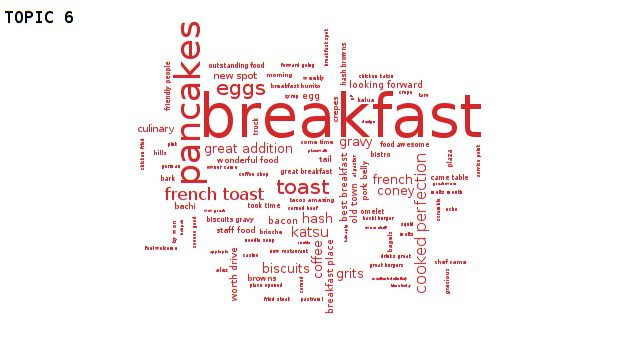
\includegraphics[width=0.35\textwidth]{./img/pos_reviews/pos_topic6.png} }
  \subfigure[Topic 7] { 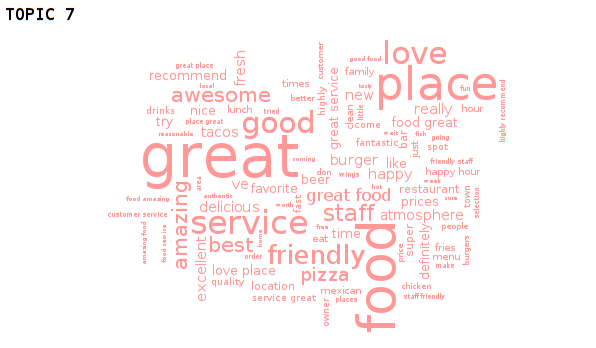
\includegraphics[width=0.35\textwidth]{./img/pos_reviews/pos_topic7.png} }
  \subfigure[Topic 8] { 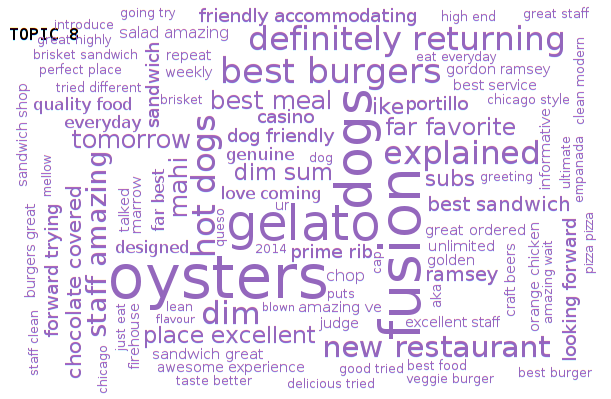
\includegraphics[width=0.35\textwidth]{./img/pos_reviews/pos_topic8.png} }
  \subfigure[Topic 9] { 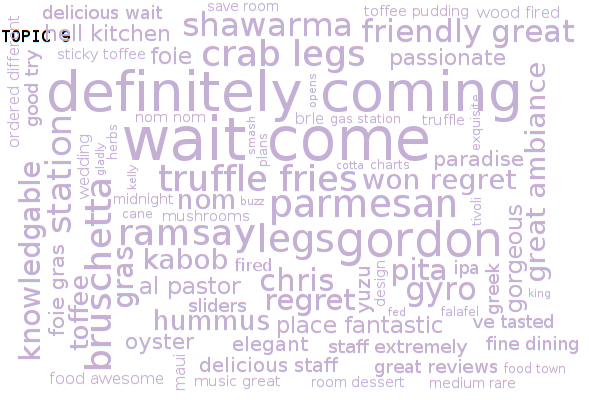
\includegraphics[width=0.35\textwidth]{./img/pos_reviews/pos_topic9.png} }
  \caption{Ten topics mined from positive restaurant reviews}
  \label{fig:pos_topics}
\end{figure}

From these results, it is shown that:
\begin{enumerate}
  \item Both positive and negative reviews still talk much about food or cuisines themselves frequently. For instance, in negative review topics, tacos, crab legs, sushi, carne asada, pizza, hot dogs are the top topics. While for positive reviews, still pizza, sushi, Indian food, chicken, breakfast, oysters are mentioned.
  \item Compared with all reviews, these subsets now shows something different in different subsets.
    \begin{itemize}
      \item In the positive review topics, there is no negative impression when looking at the top words in each word cloud of each topic. And even for the positive topics, the phrasing are quite general (``great place'', ``amazing'', ``definitely coming'') and not touching specific factors that influence customers' rating.
      \item However in the negative review topics, many specific terms indicate what the customers are looking for -- ``portion size'', ``short ribs'', ``limited menu'', ``service'', ``time'', i.e. amount of food, menues, service, and time. At the same time, general comments (e.g. ``just okay'') can still be seen.
    \end{itemize}
\end{enumerate}


\subsection{Topic mining of reviews from different cuisines}
Since reviews are made to different restaurants, and different restaurants do have different categories, or cuisines. Intuitively, one could imagine the topics mentioned in the reviews could vary.

Here I did some topic extraction upon reviews from different categories, and hereby present the comparison between category ``Automotive'', ``Tours'', and ``Seafood Market''.

Figure \ref{fig:sub_topics} shows a collection of all three categories, 2 topics sampled for each.

The result is also shown in
\href{http://jiacheng-pan.me/standalone/datamining_capstone/task1/auto_reviews_topics.html}{Automotive},
\href{http://jiacheng-pan.me/standalone/datamining_capstone/task1/sea_reviews_topics.html}{Seafood Markets},
and 
\href{http://jiacheng-pan.me/standalone/datamining_capstone/task1/tour_reviews_topics.html}{Tours}.

\begin{figure}[htp!]
  \centering
  \subfigure[Automotive Topic 0] { 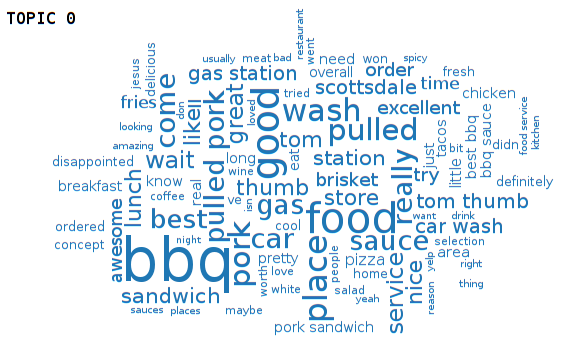
\includegraphics[width=0.35\textwidth]{./img/sub_reviews/auto_topic0.png} }
  \subfigure[Automotive Topic 4] { 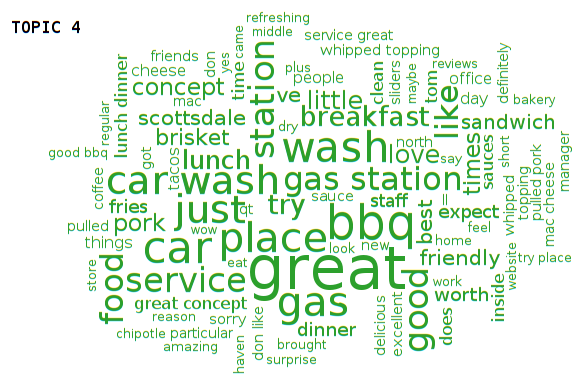
\includegraphics[width=0.35\textwidth]{./img/sub_reviews/auto_topic4.png} }
  \subfigure[Seafood Market Topic 0] { 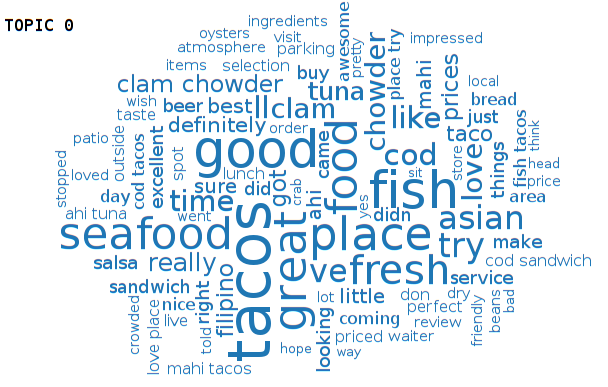
\includegraphics[width=0.35\textwidth]{./img/sub_reviews/sea_topic0.png} }
  \subfigure[Seafood Market Topic 3] { 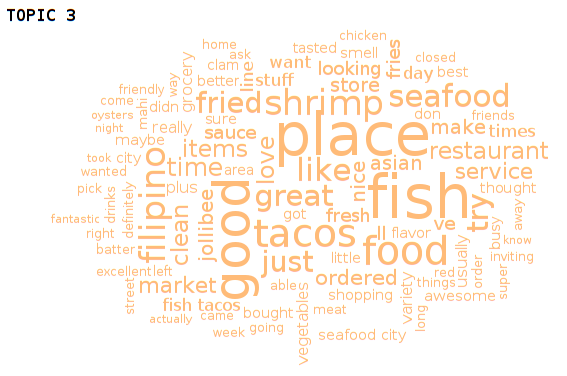
\includegraphics[width=0.35\textwidth]{./img/sub_reviews/sea_topic3.png} }
  \subfigure[Tours Topic 0] { 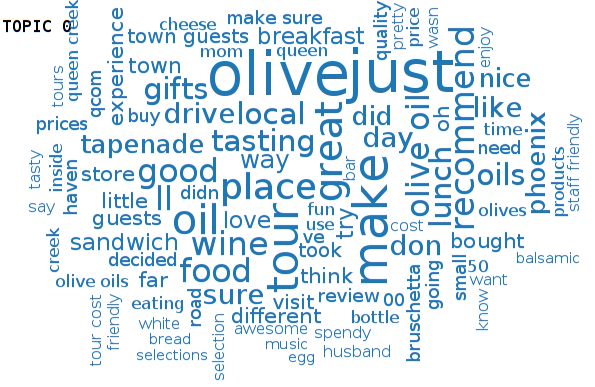
\includegraphics[width=0.35\textwidth]{./img/sub_reviews/tour_topic0.png} }
  \subfigure[Tours Topic 4] { 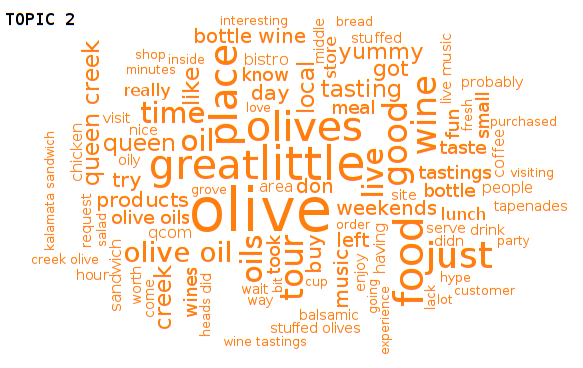
\includegraphics[width=0.35\textwidth]{./img/sub_reviews/tour_topic.png} }
  \caption{Ten topics mined from reviews of categories ``Automotive'', ``Seafood Market'', and ``Tours''}
  \label{fig:sub_topics}
\end{figure}

As is shown, although food is still the popular topic, there indeed are some divergences among the three categories:
\begin{enumerate}
  \item The food mentioned are different, of course. (BBQ for automotive, fish and shrimps for seafood, and olive oil for tours.)
  \item In particular, speciality of the restaurants are reflected in the reviews. Especially, in the automotive category, ``car wash'' and ``gas station'' are mentioned frequently. And it is understandable -- a restaurant that is relevant to automotives, is very likely to be a restaurant near a gas station, or some automotive service stations.
\end{enumerate}

\subsection{Exploration of the star distribution}
As is mentioned in the observation of Task 1.1, the topics extracted shows that at least two of them indicate a general positive impression, while only one mentioned ``time'', which might potentially reflect some neutral or negative impression.

So I then become curious about how the positions of all the reviews distribute -- do people tend to comment positively or evenly?

I choose to observe star distribution to examine this topic.

Figure \ref{fig:star_dist} shows how reviews of 1-5 stars distribute.

\begin{figure}[htp!]
  \centering
  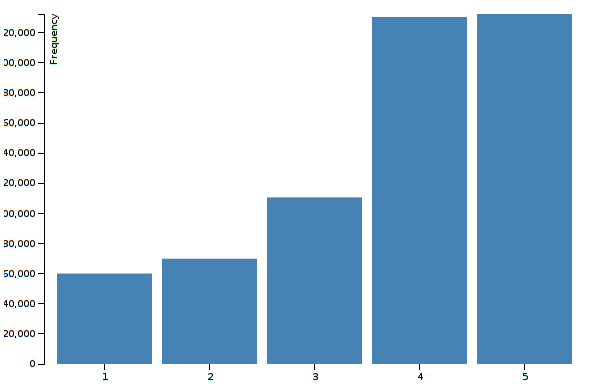
\includegraphics[width=0.8\textwidth]{./img/star_dist.png}
  \caption{Ten topics mined from positive restaurant reviews}
  \label{fig:star_dist}
\end{figure}

As is shown, the reviews are highly skewed, where positive reviews takes majority of all reviews.


\end{document}
